\section{Results}
\label{sec:results}

\subsection{Held-out Berka: the primary result}
Table~\ref{tab:heldout} gives every method on the
\R{ho/data/accounts_with_eligible_origin} held-out accounts with eligible
origins (\R{ho/data/eligible_origins} origins, each forecast at three
horizons).

\begin{table}[t]
\centering\footnotesize\setlength{\tabcolsep}{4pt}
\tab{heldout-main}
\caption{Held-out Berka. Coverage of central intervals (\%), mean CRPS skill
against B-SA+ (positive: better than B-SA+), and the share of PIT values in
the outer two of ten bins (\%; a flat histogram puts a fifth of the values there). Columns are
horizons in days. V2, in bold, is the frozen primary model. Bootstrap
intervals for every cell are in the result files; for skill they are
narrow (Table~\ref{tab:pairwise}).}
\label{tab:heldout}
\end{table}

\paragraph{Calibration (claim A2): fails at the \lA\% level.} V2's \lC\%
interval covers \R{ho/var/V2/7/cov90}, \R{ho/var/V2/30/cov90} and
\R{ho/var/V2/90/cov90}\% at \hA, \hB\ and \hC\ days, and its \lD\% interval
\R{ho/var/V2/7/cov95}, \R{ho/var/V2/30/cov95} and \R{ho/var/V2/90/cov95}\%;
all of these pass. The \lA\% interval covers \R{ho/var/V2/7/cov50}\%
[\R{ho/var/V2/7/cov50_lo}, \R{ho/var/V2/7/cov50_hi}],
\R{ho/var/V2/30/cov50}\% and \R{ho/var/V2/90/cov50}\%. Each of these
bootstrap intervals lies wholly outside the band, so those cells fail. So
does the \lB\% interval at \hB\ days, at \R{ho/var/V2/30/cov80}\%
[\R{ho/var/V2/30/cov80_lo}, \R{ho/var/V2/30/cov80_hi}]. The PIT histograms
(Figure~\ref{fig:pit}) are hump-shaped at \hB\ and \hC\ days: V2's cone is
too wide in its middle. This is the opposite of V0's failure. V0 covers
\R{ho/var/V0/30/cov90}\% and \R{ho/var/V0/90/cov90}\% at the \lC\% level,
and its PIT is U-shaped. The selection rule tested the \lC\% level only,
which is why a variant that misses the \lA\% level was selected.

\begin{figure}[t]
\centering
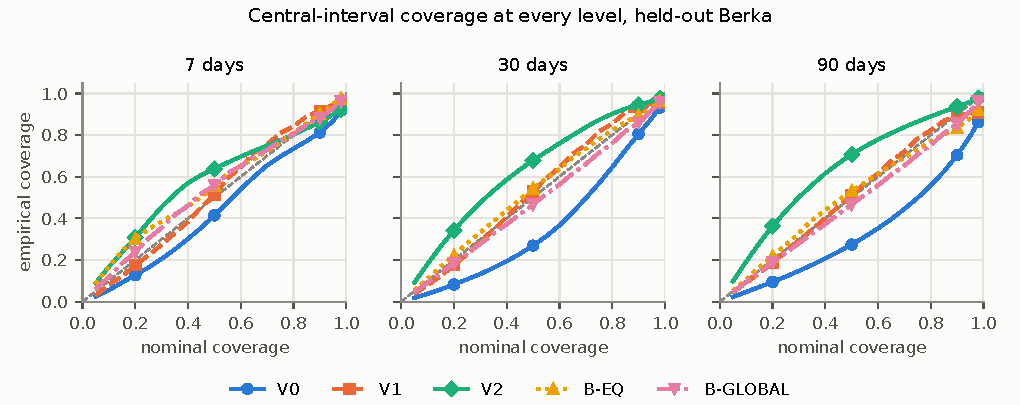
\includegraphics[width=\linewidth]{figures/coverage-heldout.pdf}
\caption{Empirical against nominal coverage of central intervals at every
level of a fine grid, held-out Berka. Points on the diagonal are
calibrated.}
\label{fig:coverage}
\end{figure}

\begin{figure}[t]
\centering
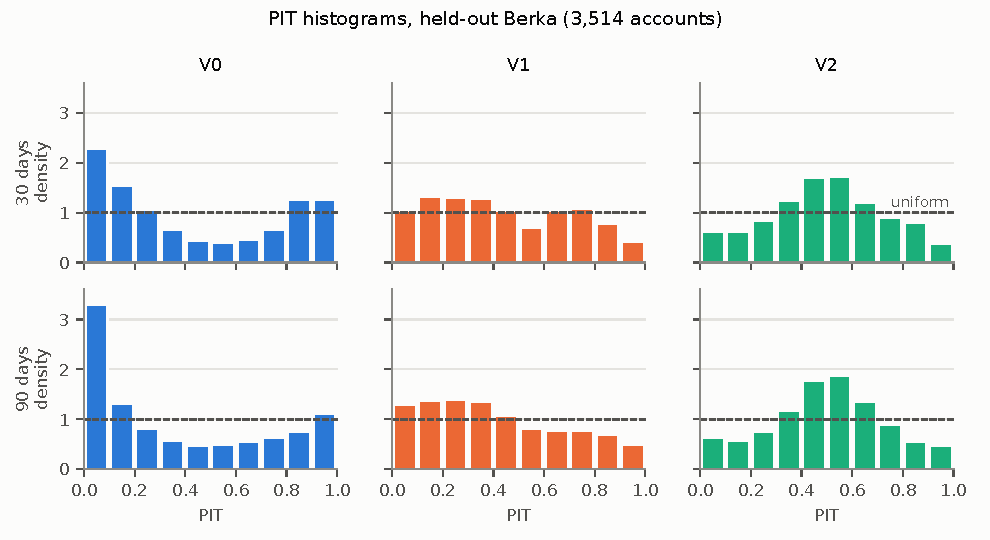
\includegraphics[width=0.85\linewidth]{figures/pit-heldout.pdf}
\caption{PIT histograms on held-out Berka. Flat is calibrated; U-shaped is
too narrow (V0); hump-shaped is too wide (V2).}
\label{fig:pit}
\end{figure}

\paragraph{Sharpness (claim B1): passes against B-SA+, fails against B-EQ
and B-GLOBAL.} Figure~\ref{fig:skill} and Table~\ref{tab:pairwise} (Appendix) compare
V2 with each baseline on the forecasts both made. Against B-SA+, the
baseline the plan named as the one that matters, V2's skill is
\R{ho/pair/B-SA+/30/skill} [\R{ho/pair/B-SA+/30/skill_lo},
\R{ho/pair/B-SA+/30/skill_hi}] at \hB\ days and \R{ho/pair/B-SA+/90/skill} at
\hC. It also beats B-30, B-LIN, B-SA and B-SEAS at both horizons. Against
B-EQ, it is \R{ho/pair/B-EQ/30/skill} [\R{ho/pair/B-EQ/30/skill_lo},
\R{ho/pair/B-EQ/30/skill_hi}] and \R{ho/pair/B-EQ/90/skill}. Against
B-GLOBAL, it is \R{ho/pair/B-GLOBAL/30/skill} and
\R{ho/pair/B-GLOBAL/90/skill}. The plan predicted no significant
difference at \hA\ days; that prediction was wrong too. V2 is significantly
better than every baseline except B-GLOBAL there, and significantly worse
than B-GLOBAL.
\begin{figure}[t]
\centering
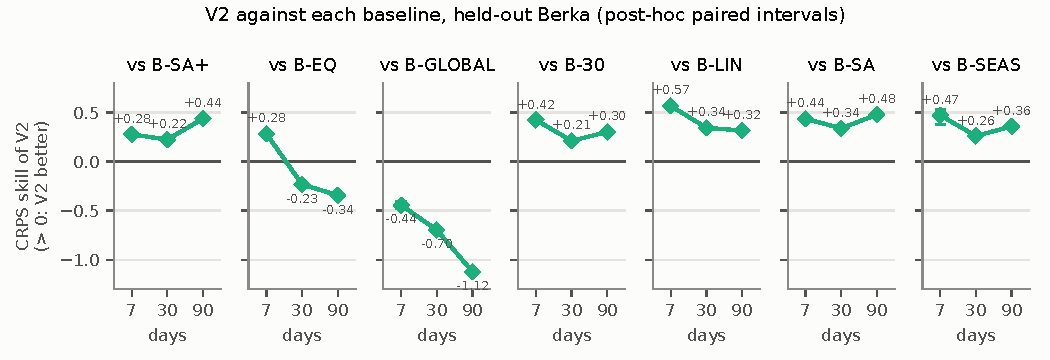
\includegraphics[width=\linewidth]{figures/skill-v2-heldout.pdf}
\caption{V2's CRPS skill against each baseline by horizon (held-out, post
hoc paired intervals).}
\label{fig:skill}
\end{figure}

B-GLOBAL learns from \R{dev/data/accounts_run} other accounts; the
local-first design cannot do that, so its win marks what pooling buys, not
a competitor the design could have used. B-EQ is the result that matters
more. It uses only the account's own history, exactly as the model does,
and it is sharper at \hB\ and \hC\ days. A simple empirical forecast of
the account's own balance changes is the better per-account forecaster on
Berka at those horizons. B-EQ is not uniformly better: its \lC\% interval
covers \R{ho/var/B-EQ/90/cov90}\% at \hC\ days, and on accounts with under a
year of history only \R{ho/str/history-lt-12-months/B-EQ/90/cov90}\%,
against V2's \R{ho/str/history-lt-12-months/V2/90/cov90}\%
(Table~\ref{tab:strata}).

\paragraph{Strata.} V2's skill against B-SA+ is positive in every stratum
(Table~\ref{tab:strata}): with and without detected income, at every
history length, and after an alarm. The lowest is \R{d/v2-strata-skill-90-min} at \hC\ days. Its \lC\% coverage at
\hC\ days ranges from \R{d/v2-strata-cov90-90-min} to
\R{d/v2-strata-cov90-90-max}\% across strata. Without detected
income, the model has no income term; there V2's \hC-day skill is
\R{ho/str/no-income-detected/V2/90/skill}, but B-EQ's is higher still
(\R{ho/str/no-income-detected/B-EQ/90/skill}).
\subsection{Development and held-out agree}
V2 on held-out data matches its development numbers
(Table~\ref{tab:devho}). Coverage differs by at most
\R{d/v2-devho-cov-maxdiff} points at any level and horizon, and skill by at
most \R{d/v2-devho-skill-maxdiff}. The selection rule applied to the
held-out results would choose V2 again; V2's worst \lC\%-coverage error
there is \R{d/ho-v2-worst90} points. There is no sign that the revision
overfitted the development split. This is unsurprising, because the
revision has few free parameters. It also means the held-out failures above
were already visible on development: the hump-shaped PIT and the losses to
B-EQ and B-GLOBAL. The plan's selection rule did not look at them.
\subsection{V1 is the best-calibrated variant}
The conformal recalibration of V0 brings every level near nominal
(Figure~\ref{fig:coverage}). On held-out data, V1's \lA\% interval covers
\R{ho/var/V1/7/cov50}, \R{ho/var/V1/30/cov50} and \R{ho/var/V1/90/cov50}\%,
and its \lC\% interval \R{ho/var/V1/7/cov90}, \R{ho/var/V1/30/cov90} and
\R{ho/var/V1/90/cov90}\%. Its PIT is nearly flat. It lost the selection on
CRPS: its skill against B-SA+ is \R{ho/var/V1/30/skill} and
\R{ho/var/V1/90/skill} at \hB\ and \hC\ days, against V2's
\R{ho/var/V2/30/skill} and \R{ho/var/V2/90/skill}. A user who cares about
every quantile, not just the \lC\% band, would be better served by V1.

\subsection{Synthetic data}
\paragraph{Claim A1 holds.} On model-matched data, with the protocol of the
engine's earlier calibration test, every central interval of V0 is within
the tolerance at every horizon (Appendix, Table~\ref{tab:a1}). With the
detector off, the \lC\% interval covers \R{syn/a1/no-detector/7/0.9/coverage},
\R{syn/a1/no-detector/30/0.9/coverage} and
\R{syn/a1/no-detector/90/0.9/coverage}\%. This is a correctness check: on
data drawn from its own model the filter is the right estimator, and
passing says little about usefulness.

\paragraph{The synthetic panel (claim B2).} Table~\ref{tab:synthetic}
gives \R{c/panel-seeds} seeds of \R{c/panel-days} days per generator. V2's
sparse rule never fired on synthetic data (\R{d/syn-sparse} of
\R{d/syn-origins} origins), because synthetic spending has many small
transactions a day. So V2 equals V0 here, and synthetic data says nothing
about V2's sparse model, which is exercised only on Berka. There the rule
fired at every one of \R{ho/vdata/origins} held-out origins. On the
realistic generator, V0 beats B-SA+ (skill \R{syn/re/V0/30/skill} and
\R{syn/re/V0/90/skill} at \hB\ and \hC\ days) and every per-account
baseline. Against B-GLOBAL, trained on \R{c/train-seeds} separate seeds of
the same generator, it ties: paired skill \R{syn/rep/V0/B-GLOBAL/30/skill}
[\R{syn/rep/V0/B-GLOBAL/30/skill_lo}, \R{syn/rep/V0/B-GLOBAL/30/skill_hi}]
and \R{syn/rep/V0/B-GLOBAL/90/skill}
[\R{syn/rep/V0/B-GLOBAL/90/skill_lo}, \R{syn/rep/V0/B-GLOBAL/90/skill_hi}].
B2 therefore fails against B-GLOBAL. On model-matched data B-GLOBAL even
wins at \hB\ days (\R{syn/mmp/V0/B-GLOBAL/30/skill}).

\begin{table}[t]
\centering\footnotesize
\tab{synthetic-main}
\caption{Synthetic panel: coverage (\%) and skill against B-SA+. V2's
sparse rule never fired, so V2 equals V0. V3 was not run on synthetic
data.}
\label{tab:synthetic}
\end{table}

\paragraph{The B-EQ reversal.} B-EQ, the strongest per-account baseline on
Berka, loses clearly to B-SA+ on synthetic data. Its skill against B-SA+
on the realistic generator is \R{syn/re/B-EQ/30/skill} at \hB\ days,
against \R{ho/var/B-EQ/30/skill} on held-out Berka. We have not tested why. A
plausible reading is that synthetic accounts have a strong, regular pay
cycle, which the schedule-aware methods use and an unconditional
distribution of past changes blurs. Berka balances move in a few large,
irregular steps. The reversal is itself a warning: a method's ranking on
our own generator did not predict its ranking on real data.

\subsection{MoneyData: one account, descriptive}
On the single MoneyData account (Table~\ref{tab:moneydata} in the
Appendix; \R{md/data/eligible_origins} weekly origins), V0 is badly
miscalibrated. Its \lC\% interval covers \R{md/main/V0/7/cov90},
\R{md/main/V0/30/cov90} and \R{md/main/V0/90/cov90}\%. V1's recalibration
brings this to \R{md/main/V1/7/cov90}, \R{md/main/V1/30/cov90} and
\R{md/main/V1/90/cov90}\%, and B-EQ has the best CRPS. About
\R{d/md-irregular-share}\% of the account's gross flow is one-off: inflows
of up to \pounds\R{d/md-largest-inflow}, an account transfer of
\pounds\R{d/md-transfer}, and investment purchases. The model has no term
for such flows. V2's sparse rule did not fire on this account, which has
\R{md/data/records_per_month} records a month, so V2 equals V0 here too. We
draw no general conclusion from one account. Figure~\ref{fig:cone} (Appendix) shows an example
forecast on a Berka development account.
